\begin{problem}%
{У вас течёт!}%
{\textsl{стандартный ввод}}%
{\textsl{стандартный вывод}}%
{2 секунды}%
{256 мегабайт}%
{}

Где-то в Москве в очередной раз построили новый дом: красивый, современный и многоэтажный. Он состоит из ровно $n$ жилых этажей, пронумерованных от $1$ до $n$ снизу вверх, и подземной парковки, являющейся нулевым этажом.\\

Дом уже был почти готов к сдаче в эксплуатацию, но вот незадача — в самый ответственный момент по всему зданию прорвало водопроводные трубы, в результате чего многие этажи залило водой. К моменту, когда все трубы были заделаны, на $i$-м этаже находилось $w_i$ литров воды.\

Также из-за того, что при строительстве дома все средства ушли на отделку фасада, а на перекрытия между этажами был пущен самый дешёвый материал, оказалось, что между этажами ощутимо протекают потолки. В частности, пропускная способность пола $i$-го этажа составляет $v_i$ литров воды в час.\\

В рамках данной задачи считается, что скорость вытекания воды с этажа зависит только от пропускной способности пола и не зависит от количества воды на этаже. Временем падения воды с потолка этажа до пола также следует пренебречь. Считайте, что все этажи достаточно объёмные, чтобы вместить всю воду, скопившуюся в здании.\\

Владельцы стройки интересуются, через сколько часов вся вода вытечет на парковку, и они смогут начать продажи квартир?

\InputFile

В первой строке записано единственное целое число $n$ ($1 \le n \le 200000$) — количество жилых этажей здания.\\

Вторая строка содержит $n$ целых чисел $w_1$, $w_2$, ..., $w_n$ ($0 \le w_i \le 1000$) , задающих количество воды в литрах на каждом из жилых этажей здания.\\

Третья строка содержит $n$ целых чисел $v_1$, $v_2$, ..., $v_n$ ($1 \le v_i \le 200000$), задающих скорость протекания пола каждого из жилых этажей здания в литрах в час.

\OutputFile

Выведите единственное число — время в часах, через которое вся вода стечёт на подземную парковку.\\

Ваш ответ будет засчитан, если его абсолютная или относительная погрешность не превосходит $10^{-4}$, а именно: если ваш ответ - $p_{ans}$, а ответ жюри - $j_{ans}$, то ваш ответ будет засчитан, если $\frac{\abs{p_{ans} - j_{ans}}}{max(1, \abs{j_{ans}})} \le 10^{-4}$ .

\Examples

\begin{example}
\exmp{
2
10 20
5 5
}{%
6.0000000000
}%
\exmp{
3
0 0 100
45 40 50
}{%
2.5000000000
}%
\end{example}

\Explanation

В первом примере на первом этаже изначально $10$ литров воды, а на втором — $20$ литров, все полы текут со скоростью $5$ литров в час. Через $2$ часа после начала $10$ единиц воды перетечёт с первого этажа на парковку, а также со второго этажа на первый, значит, на первом этаже количество воды не изменится, а на втором этаже станет на $10$ литров меньше. По прошествии ещё двух часов на первом этаже по-прежнему будет $10$ литров воды, а второй этаж опустеет. А ещё через $2$ часа вся вода с первого этажа стечёт на подземную парковку.

\begin{center}
\begin{adjustbox}{max size={\textwidth}{\textheight}}
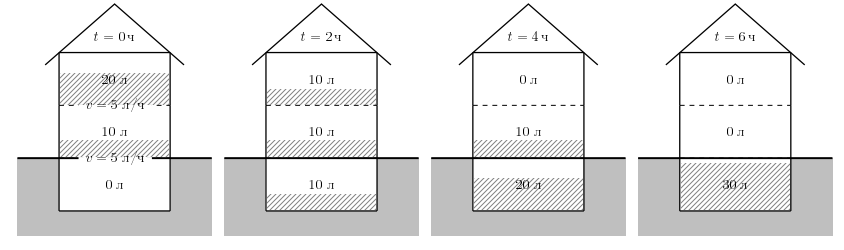
\includegraphics{images/2966.png}
\end{adjustbox}
\end{center}

Во втором примере через два часа после начала на третьем этаже совсем не останется воды. За это же время из $100$ литров, притёкших на второй этаж, останется только $20$, а $80$ литров, перетёкших со второго этажа на первый, сразу окажутся на парковке, потому что пропускная способность пола на первом этаже выше, чем пропускная способность потолка (являющегося полом второго этажа). За полчаса оставшийся объём воды на втором этаже перетечёт на первый этаж и сразу окажется на парковке, таким образом, ответ — $2.5$ часа.

\begin{center}
\begin{adjustbox}{max size={\textwidth}{\textheight}}
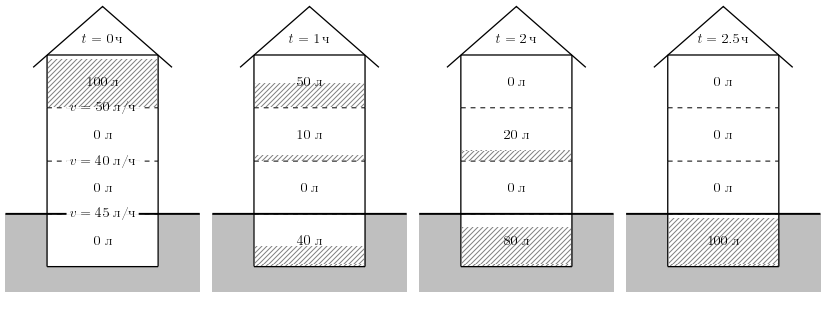
\includegraphics{images/2967.png}
\end{adjustbox}
\end{center}

\end{problem}